\section{Các phép toán và Lọc ảnh cơ bản}
\label{sec:basic_image_operations_filtering}

\subsection{Giới thiệu: Thao tác trên Lưới Pixel}
\label{subsec:filtering_intro}

Một hình ảnh kỹ thuật số, như chúng ta đã tìm hiểu, là một ma trận số khổng lồ. Để trích xuất thông tin có ý nghĩa từ ma trận này, chúng ta cần các công cụ để thao tác, biến đổi, và làm nổi bật các cấu trúc quan trọng. Các phép toán và lọc ảnh cơ bản chính là bộ công cụ nền tảng đó. Chúng là những thao tác ở cấp độ thấp, hoạt động trực tiếp trên các giá trị pixel và các vùng lân cận của chúng, nhưng lại là tiền đề cho hầu hết các tác vụ thị giác phức tạp hơn.

Trong phần này, chúng ta sẽ khám phá một trong những khái niệm mạnh mẽ và phổ quát nhất trong toàn bộ lĩnh vực xử lý tín hiệu và thị giác máy tính: \textbf{phép tích chập (convolution)}. Phép toán tưởng chừng đơn giản này—một thao tác "trượt và nhân"—lại là trái tim của vô số ứng dụng:
\begin{itemize}
    \item \textbf{Làm mờ ảnh (Blurring):} Bằng cách lấy trung bình các pixel lân cận, chúng ta có thể loại bỏ nhiễu và làm mịn các chi tiết, một bước tiền xử lý quan trọng.
    \item \textbf{Làm sắc nét ảnh (Sharpening):} Bằng cách nhấn mạnh sự khác biệt giữa một pixel và các lân cận của nó, chúng ta có thể làm cho các cạnh và chi tiết trở nên rõ ràng hơn.
    \item \textbf{Phát hiện biên (Edge Detection):} Bằng cách thiết kế các bộ lọc (kernels) chuyên dụng, chúng ta có thể tìm ra những nơi có sự thay đổi đột ngột về cường độ sáng, qua đó phác họa nên "bộ xương" cấu trúc của các đối tượng trong ảnh.
\end{itemize}

Việc nắm vững các kỹ thuật này không chỉ cung cấp một bộ công cụ thực hành để xử lý ảnh, mà còn xây dựng một trực giác sâu sắc về cách các thông tin cục bộ có thể được tổng hợp để tạo ra các nhận định toàn cục hơn. Điều quan trọng hơn, khái niệm về tích chập và kernel chính là nguồn cảm hứng trực tiếp và là nền tảng toán học cho các lớp tích chập trong Mạng Nơ-ron Tích chập (CNN), trái tim của cuộc cách mạng học sâu. Hiểu rõ tích chập cổ điển là bước đệm không thể thiếu để thấu hiểu cách CNN "học" cách nhìn thế giới.

\subsection{Phép Tích chập (Convolution) và Nhân (Kernel)}
\label{subsec:convolution_and_kernel}

Phép tích chập là một phép toán toán học được định nghĩa cho hai hàm số, tạo ra một hàm thứ ba biểu diễn "sự chồng chéo" có trọng số của hai hàm khi một hàm được dịch chuyển qua hàm kia. Trong xử lý ảnh, nó được đơn giản hóa thành một phép toán rời rạc giữa một ma trận ảnh và một ma trận nhỏ hơn gọi là \textbf{nhân (kernel)} hay \textbf{bộ lọc (filter)}.

\subsubsection{Định nghĩa Toán học của Tích chập 2D}
\label{subsubsec:convolution_definition}
Cho một ảnh đầu vào $\mathbf{I}$ và một kernel $\mathbf{K}$ có kích thước $(2k+1) \times (2k+1)$, giá trị của ảnh đầu ra $\mathbf{G}$ tại vị trí pixel $(i, j)$ được tính bằng phép tích chập 2D rời rạc:
\begin{equation}
    \mathbf{G}(i, j) = (\mathbf{I} * \mathbf{K})(i, j) = \sum_{u=-k}^{k} \sum_{v=-k}^{k} \mathbf{K}(u, v) \mathbf{I}(i-u, j-v)
    \label{eq:convolution}
\end{equation}
\textbf{Trực giác của công thức:}
Công thức trên mô tả một quá trình "trượt và nhân". Để tính giá trị cho một pixel đầu ra tại $(i,j)$, chúng ta thực hiện các bước sau:
\begin{enumerate}
    \item \textbf{Lật kernel:} Lật kernel $\mathbf{K}$ theo cả chiều ngang và chiều dọc. Đây là định nghĩa toán học chuẩn của tích chập. Tuy nhiên, trong thực tế xử lý ảnh và học sâu, bước này thường được bỏ qua (hoặc kernel được giả định là đối xứng), và phép toán được gọi chính xác hơn là \textbf{tương quan chéo (cross-correlation)}:
    \begin{equation}
        \mathbf{G}(i, j) = \sum_{u=-k}^{k} \sum_{v=-k}^{k} \mathbf{K}(u, v) \mathbf{I}(i+u, j+v)
        \label{eq:cross_correlation}
    \end{equation}
    Trong suốt cuốn sách này, khi nói về "tích chập" trong ngữ cảnh của CNN, chúng ta sẽ ngầm hiểu đó là phép tương quan chéo, vì đây là cách nó được triển khai trong tất cả các thư viện học sâu hiện đại.
    
    \item \textbf{Đặt kernel:} Đặt tâm của kernel (đã lật hoặc không) lên trên pixel $(i, j)$ của ảnh đầu vào.
    
    \item \textbf{Nhân và Tổng hợp:} Thực hiện phép nhân từng phần tử (element-wise multiplication) giữa các giá trị của kernel và các giá trị pixel của ảnh đầu vào nằm bên dưới nó.
    
    \item \textbf{Gán giá trị:} Tổng của tất cả các tích này chính là giá trị của pixel đầu ra $\mathbf{G}(i, j)$.
    
    \item \textbf{Lặp lại:} Lặp lại quá trình này cho tất cả các pixel $(i, j)$ trên ảnh đầu vào để tạo ra ảnh đầu ra hoàn chỉnh.
\end{enumerate}

\begin{center}
    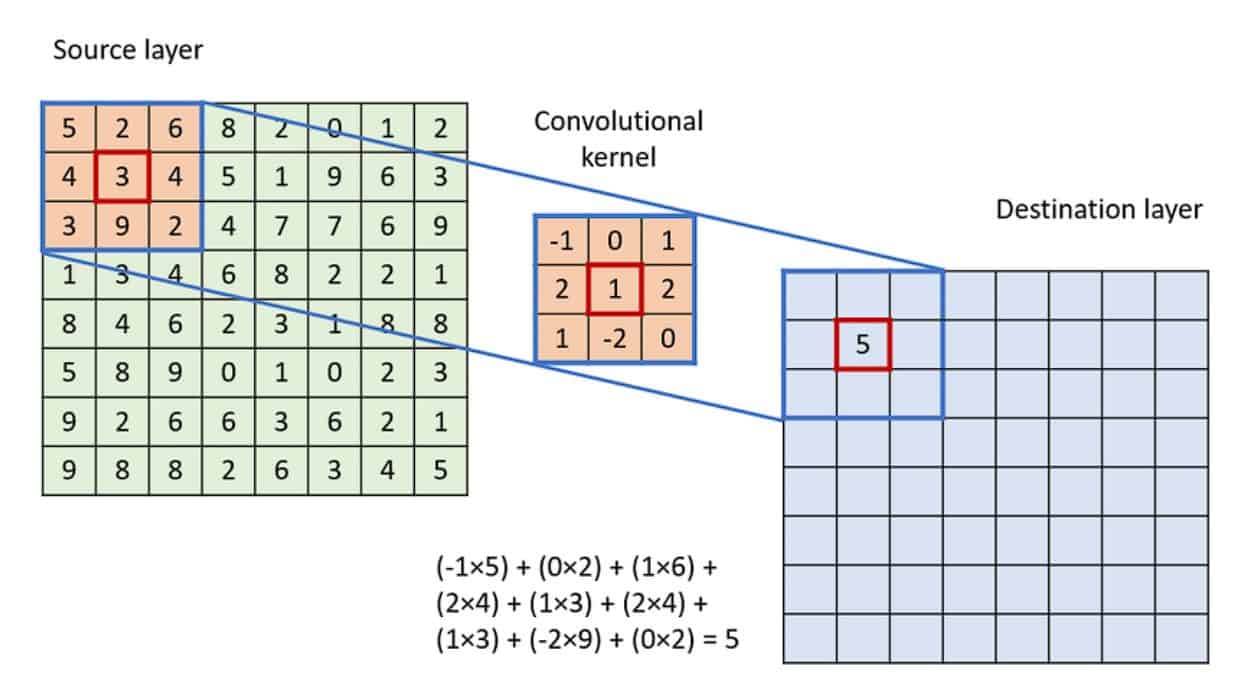
\includegraphics[width=1.0\textwidth]{images/convolution_detailed.jpg}
    \captionof{figure}{Minh họa chi tiết một bước của phép tương quan chéo 2D (thường được gọi là tích chập trong học sâu).}
    \label{fig:convolution_detailed}
\end{center}

\subsubsection{Các tham số quan trọng: Padding và Stride}
\label{subsubsec:padding_stride}
Khi thực hiện tích chập, có hai siêu tham số quan trọng quyết định kích thước và nội dung của ảnh đầu ra.
\begin{description}
    \item[Padding (Đệm):] Phép tích chập chỉ có thể được tính toán tại những vị trí mà kernel nằm hoàn toàn bên trong ảnh. Điều này có nghĩa là ảnh đầu ra sẽ bị thu nhỏ lại so với ảnh đầu vào. Ví dụ, một ảnh $5 \times 5$ tích chập với kernel $3 \times 3$ sẽ tạo ra một ảnh $3 \times 3$. Sự co lại này, đặc biệt trong các mạng nơ-ron sâu với nhiều lớp, sẽ làm mất thông tin không gian rất nhanh và bỏ qua thông tin quan trọng ở các pixel rìa.
    
    \textbf{Giải pháp:} Thêm một đường viền gồm các pixel (thường là giá trị 0) xung quanh ảnh đầu vào. Kỹ thuật này được gọi là \textbf{zero-padding}.
    \begin{itemize}
        \item \textbf{`valid` padding:} Không sử dụng padding. Kích thước đầu ra bị giảm.
        \item \textbf{`same` padding:} Sử dụng một lượng padding vừa đủ để kích thước của ảnh đầu ra bằng với kích thước của ảnh đầu vào. Với kernel kích thước $F \times F$, lượng padding cần thêm vào mỗi bên là $P = (F-1)/2$. Điều này đòi hỏi $F$ phải là số lẻ.
    \end{itemize}
    
    \item[Stride (Bước nhảy):] Tham số này xác định khoảng cách mà kernel dịch chuyển trên ảnh đầu vào sau mỗi lần tính toán.
    \begin{itemize}
        \item \textbf{Stride = 1:} Kernel dịch chuyển 1 pixel mỗi lần. Đây là trường hợp phổ biến nhất.
        \item \textbf{Stride > 1:} Kernel nhảy qua các pixel. Điều này có tác dụng \textbf{giảm kích thước (downsampling)} của ảnh đầu ra. Một tích chập với stride bằng 2 sẽ làm giảm kích thước của feature map đi một nửa.
    \end{itemize}
\end{description}

Kích thước của ảnh đầu ra ($W_{out}, H_{out}$) có thể được tính từ kích thước ảnh đầu vào ($W_{in}, H_{in}$), kích thước kernel ($F$), padding ($P$), và stride ($S$) theo công thức:
\begin{equation}
    W_{out} = \frac{W_{in} - F + 2P}{S} + 1
\end{equation}

\subsubsection{Mã nguồn Python: Tích chập 2D với NumPy}
\label{subsubsec:convolution_python}
Để hiểu rõ hơn, chúng ta có thể tự triển khai một phép tích chập 2D đơn giản bằng NumPy.
\begin{minted}[fontsize=\footnotesize, frame=single, linenos=true]{python}
import numpy as np

def convolve2d(image, kernel, stride=1, padding=0):
    """
    Trien khai phep tuong quan cheo 2D (convolution trong hoc sau).
    Implementation of 2D cross-correlation (convolution in deep learning).
    """
    # Lat kernel 180 do cho phep tich chap toan hoc chuan, nhung thuong duoc bo qua
    # kernel = np.flipud(np.fliplr(kernel))

    # Kich thuoc cua kernel va anh
    kernel_h, kernel_w = kernel.shape
    image_h, image_w = image.shape

    # Them padding vao anh
    if padding > 0:
        padded_image = np.pad(image, ((padding, padding), (padding, padding)), mode='constant')
    else:
        padded_image = image
    
    padded_h, padded_w = padded_image.shape

    # Tinh kich thuoc anh dau ra
    output_h = (padded_h - kernel_h) // stride + 1
    output_w = (padded_w - kernel_w) // stride + 1
    
    # Khoi tao ma tran dau ra
    output_image = np.zeros((output_h, output_w))

    # Thuc hien phep tich chap
    for y in range(0, output_h):
        for x in range(0, output_w):
            # Tinh toan toa do bat dau va ket thuc cua vung anh
            y_start = y * stride
            y_end = y_start + kernel_h
            x_start = x * stride
            x_end = x_start + kernel_w
            
            # Trich xuat vung anh (Region of Interest - ROI)
            roi = padded_image[y_start:y_end, x_start:x_end]
            
            # Nhan tung phan tu va tinh tong
            output_image[y, x] = np.sum(roi * kernel)
            
    return output_image

# --- Vi du su dung ---
# Anh dau vao
input_image = np.array([
    [1, 1, 1, 0, 0],
    [0, 1, 1, 1, 0],
    [0, 0, 1, 1, 1],
    [0, 0, 1, 1, 0],
    [0, 1, 1, 0, 0]
])

# Kernel phat hien canh doc
sobel_x = np.array([
    [-1, 0, 1],
    [-2, 0, 2],
    [-1, 0, 1]
])

# Thuc hien tich chap
output = convolve2d(input_image, sobel_x, stride=1, padding=1)

print("Anh dau vao:\n", input_image)
print("\nKernel Sobel X:\n", sobel_x)
print("\nAnh dau ra (sau khi tich chap):\n", output)
\end{minted}

\subsection{Làm mờ ảnh (Image Blurring): Loại bỏ Nhiễu và Làm mịn Chi tiết}
\label{subsec:image_blurring}
Làm mờ, hay làm mịn (smoothing), là một trong những phép lọc ảnh cơ bản và phổ biến nhất. Về bản chất, nó là một phép lọc thông thấp (low-pass filtering), có tác dụng loại bỏ các thành phần tần số cao (nhiễu, chi tiết nhỏ) và giữ lại các thành phần tần số thấp (cấu trúc tổng thể).

\subsubsection{Bộ lọc Hộp (Box Filter / Averaging Filter)}
\label{subsubsec:box_filter}
Đây là cách làm mờ đơn giản nhất. Nó hoạt động bằng cách thay thế giá trị của mỗi pixel bằng giá trị trung bình của các pixel trong một vùng lân cận hình chữ nhật xung quanh nó. Kernel tương ứng được gọi là bộ lọc hộp.

Một kernel hộp $3 \times 3$ được chuẩn hóa có dạng:
\begin{equation}
    \mathbf{K}_{\text{box}} = \frac{1}{9} 
    \begin{pmatrix} 
        1 & 1 & 1 \\ 
        1 & 1 & 1 \\ 
        1 & 1 & 1 
    \end{pmatrix}
\end{equation}
Hệ số $\frac{1}{9}$ dùng để chuẩn hóa, đảm bảo rằng tổng các phần tử của kernel bằng 1. Điều này giúp độ sáng tổng thể của ảnh không bị thay đổi sau khi lọc.

\textbf{Ưu điểm:} Rất nhanh để tính toán.
\textbf{Nhược điểm:} Tạo ra các artifact dạng hộp (blocky artifacts) vì nó gán trọng số bằng nhau cho tất cả các pixel trong vùng lân cận, bất kể khoảng cách của chúng đến pixel trung tâm.

\subsubsection{Bộ lọc Gaussian (Gaussian Blur)}
\label{subsubsec:gaussian_blur}
Bộ lọc Gaussian là phương pháp làm mờ được ưa chuộng hơn vì nó tạo ra kết quả tự nhiên và mượt mà hơn. Thay vì lấy trung bình đều, nó lấy trung bình có trọng số, trong đó các pixel ở gần trung tâm có trọng số lớn hơn các pixel ở xa. Các trọng số này được lấy từ một hàm Gaussian 2D.

Hàm Gaussian 2D có dạng:
\begin{equation}
    G(x, y) = \frac{1}{2\pi\sigma^2} e^{-\frac{x^2 + y^2}{2\sigma^2}}
    \label{eq:gaussian_2d}
\end{equation}
Trong đó:
\begin{itemize}
    \item $(x, y)$ là khoảng cách từ tâm.
    \item $\sigma$ (sigma) là độ lệch chuẩn. Đây là tham số quan trọng nhất, kiểm soát mức độ làm mờ. $\sigma$ càng lớn, ảnh càng bị mờ nhiều hơn.
\end{itemize}
Để tạo ra một kernel Gaussian rời rạc (ví dụ: $5 \times 5$), chúng ta lấy mẫu hàm $G(x, y)$ trên một lưới tọa độ nguyên $(-2, -1, 0, 1, 2)$, sau đó chuẩn hóa để tổng các phần tử bằng 1.

\begin{center}
    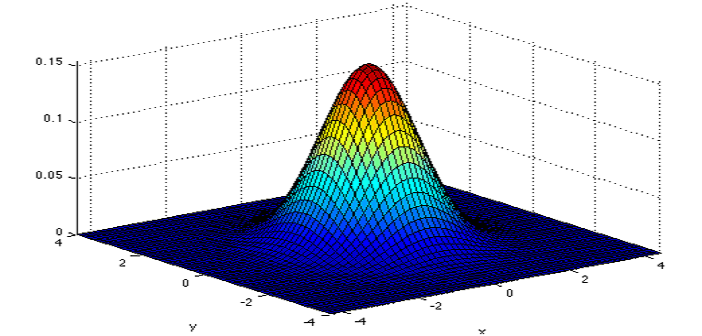
\includegraphics[width=1.0\textwidth]{images/gaussian_kernel.png}
    \captionof{figure}{Minh họa Bộ lọc Gaussian: Đồ thị 3D thể hiện hàm Gaussian 2D, cao nhất ở trung tâm và giảm dần ra các cạnh, minh họa cách các pixel gần trung tâm được nhân trọng số lớn hơn khi làm mượt ảnh.}
    \label{fig:gaussian_kernel}
\end{center}

\textbf{Tính chất quan trọng:}
\begin{itemize}
    \item \textbf{Tính tách biệt (Separability):} Một phép tích chập Gaussian 2D có thể được phân tách thành hai phép tích chập 1D: một theo chiều ngang và một theo chiều dọc. Điều này giúp giảm đáng kể độ phức tạp tính toán. Thay vì $N \times N$ phép tính cho mỗi pixel (với kernel $N \times N$), ta chỉ cần $N+N$ phép tính.
    \item \textbf{Không tạo ra cạnh giả:} Vì hàm Gaussian giảm dần một cách mượt mà, nó không tạo ra các cạnh nhân tạo như bộ lọc hộp.
\end{itemize}

\subsubsection{Ứng dụng của Làm mờ}
\label{subsubsec:blurring_applications}
\begin{itemize}
    \item \textbf{Tiền xử lý để Khử nhiễu:} Nhiễu (đặc biệt là nhiễu Gaussian) thường là các biến đổi tần số cao. Làm mờ nhẹ có thể làm giảm đáng kể nhiễu trước khi thực hiện các tác vụ khác như phát hiện biên.
    \item \textbf{Xây dựng Kim tự tháp ảnh (Image Pyramids):} Trong các thuật toán cổ điển như SIFT, ảnh được làm mờ với các mức $\sigma$ khác nhau và giảm kích thước liên tục để tạo ra một biểu diễn đa tỷ lệ, cho phép phát hiện các đặc trưng ở các kích thước khác nhau.
\end{itemize}

\subsubsection{Mã nguồn Python: Làm mờ với OpenCV}
\label{subsubsec:blurring_python}
OpenCV cung cấp các hàm được tối ưu hóa cao để thực hiện các phép lọc này.
\begin{minted}[fontsize=\footnotesize, frame=single, linenos=true]{python}
import cv2
import numpy as np
import matplotlib.pyplot as plt

try:
    # Load anh
    image = cv2.imread('noisy_image.jpg')
    if image is None:
        raise FileNotFoundError("Image not found. Please provide a sample image 'noisy_image.jpg'")
    
    image_rgb = cv2.cvtColor(image, cv2.COLOR_BGR2RGB)

    # --- 1. Lam mo voi Bo loc Hop (Averaging) ---
    # Kernel size cang lon, anh cang mo
    kernel_size_box = (15, 15)
    box_blurred = cv2.blur(image_rgb, kernel_size_box)

    # --- 2. Lam mo voi Bo loc Gaussian ---
    # Kernel size phai la so le. Sigma cang lon, anh cang mo.
    kernel_size_gaussian = (15, 15)
    sigmaX = 0 # Neu sigmaX = 0, no se duoc tinh tu kernel size
    gaussian_blurred = cv2.GaussianBlur(image_rgb, kernel_size_gaussian, sigmaX)

    # --- 3. Lam mo voi Bo loc Median ---
    # Hieu qua trong viec loai bo nhieu "muoi tieu" (salt-and-pepper noise)
    # Lay gia tri trung vi thay vi trung binh, giup bao toan canh tot hon
    median_blurred = cv2.medianBlur(image_rgb, 15)

    # --- Truc quan hoa ket qua ---
    fig, axs = plt.subplots(1, 4, figsize=(20, 5))
    axs[0].imshow(image_rgb)
    axs[0].set_title('Anh Goc')
    axs[1].imshow(box_blurred)
    axs[1].set_title('Lam mo voi Box Filter')
    axs[2].imshow(gaussian_blurred)
    axs[2].set_title('Lam mo voi Gaussian Blur')
    axs[3].imshow(median_blurred)
    axs[3].set_title('Lam mo voi Median Blur')

    for ax in axs:
        ax.axis('off')
    plt.tight_layout()
    plt.show()

except FileNotFoundError as e:
    print(e)
\end{minted}

\subsubsection{Làm sắc nét (Sharpening, Laplacian Filter)}
\label{subsec:sharpening_laplacian}

Trái ngược với làm mờ, làm sắc nét (sharpening) là một kỹ thuật nhằm làm nổi bật các chi tiết nhỏ và các đường biên trong ảnh. Về mặt xử lý tín hiệu, đây là một \textbf{phép lọc thông cao (high-pass filter)}, có nghĩa là nó làm suy yếu các thành phần tần số thấp (vùng trơn) và khuếch đại các thành phần tần số cao (cạnh, chi tiết).

\subsubsection{Cơ sở Toán học: Đạo hàm}
\label{subsubsec:sharpening_math_derivative}
Trực giác đằng sau việc làm sắc nét đến từ giải tích. Trong một tín hiệu 1D, các vùng thay đổi chậm (trơn) có đạo hàm gần bằng 0, trong khi các điểm có sự thay đổi đột ngột (cạnh) có đạo hàm với độ lớn cao. Do đó, các phép toán đạo hàm có xu hướng làm nổi bật các cạnh.
\begin{itemize}
    \item \textbf{Đạo hàm bậc nhất (First Derivative):} Cho biết tốc độ thay đổi của cường độ sáng. Tại một cạnh (step edge), đạo hàm bậc nhất có một đỉnh (peak) hoặc một đáy (valley).
    \item \textbf{Đạo hàm bậc hai (Second Derivative):} Cho biết tốc độ thay đổi của đạo hàm bậc nhất. Tại một cạnh, đạo hàm bậc hai có một điểm \textbf{cắt qua trục hoành (zero-crossing)}, tức là điểm mà giá trị của nó đổi dấu từ dương sang âm hoặc ngược lại.
\end{itemize}

\begin{center}
    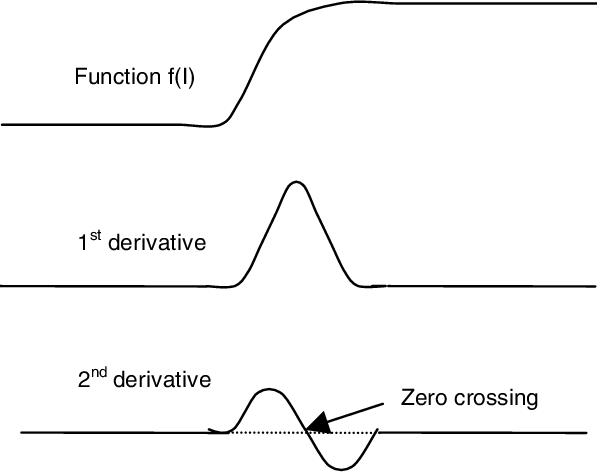
\includegraphics[width=1.0\textwidth]{images/derivative_edge_response.png}
    \captionof{figure}{Phản ứng của đạo hàm bậc nhất và bậc hai tại các loại cạnh khác nhau. (a) Một đường cắt ngang qua ảnh với các vùng cường độ khác nhau. (b) Đạo hàm bậc nhất tạo ra một đỉnh tại cạnh dốc (step edge). (c) Đạo hàm bậc hai tạo ra một điểm zero-crossing tại vị trí của cạnh và có phản ứng ở cả hai bên.}
    \label{fig:derivative_edge_response}
\end{center}

Các phép toán đạo hàm bậc hai đặc biệt hữu ích cho việc làm sắc nét vì chúng nhạy cảm hơn với các chi tiết nhỏ (như các đường mảnh và các điểm cô lập) và điểm zero-crossing của chúng cung cấp một cách định vị cạnh chính xác hơn.

\subsubsection{Toán tử Laplace (Laplacian Operator)}
\label{subsubsec:laplacian_operator}
Toán tử Laplace là một toán tử đạo hàm bậc hai trong không gian nhiều chiều. Đối với một hàm ảnh 2D $I(x, y)$, toán tử Laplace được định nghĩa là:
\begin{equation}
    \nabla^2 I = \frac{\partial^2 I}{\partial x^2} + \frac{\partial^2 I}{\partial y^2}
    \label{eq:laplacian_definition}
\end{equation}
Đây là một toán tử vô hướng (scalar), không giống như gradient là một vector. Để áp dụng trên ảnh số, chúng ta cần một phiên bản rời rạc. Sử dụng xấp xỉ sai phân trung tâm cho đạo hàm bậc hai, ta có:
\begin{align}
    \frac{\partial^2 I}{\partial x^2} &\approx I[i+1, j] - 2I[i, j] + I[i-1, j] \\
    \frac{\partial^2 I}{\partial y^2} &\approx I[i, j+1] - 2I[i, j] + I[i, j-1]
\end{align}
Cộng hai biểu thức trên lại, ta được xấp xỉ rời rạc cho toán tử Laplace:
\begin{equation}
    \nabla^2 I[i, j] \approx I[i+1, j] + I[i-1, j] + I[i, j+1] + I[i, j-1] - 4I[i, j]
    \label{eq:discrete_laplacian}
\end{equation}
Biểu thức này có thể được thực hiện bằng một phép tích chập với kernel Laplace:
\begin{equation}
    K_{\text{Laplace}} = \begin{pmatrix} 0 & 1 & 0 \\ 1 & -4 & 1 \\ 0 & 1 & 0 \end{pmatrix}
\end{equation}
Một biến thể khác của kernel Laplace cũng tính đến các lân cận chéo:
\begin{equation}
    K_{\text{Laplace\_diag}} = \begin{pmatrix} 1 & 1 & 1 \\ 1 & -8 & 1 \\ 1 & 1 & 1 \end{pmatrix}
\end{equation}
\textbf{Trực giác:} Ảnh kết quả sau khi áp dụng bộ lọc Laplace sẽ làm nổi bật các cạnh và các vùng có sự thay đổi nhanh, trong khi triệt tiêu các vùng trơn (nơi đạo hàm bậc hai gần bằng 0). Tuy nhiên, ảnh kết quả thường có nền tối và khó quan sát.

\subsubsection{Quy trình Làm sắc nét}
\label{subsubsec:sharpening_process}
Để tạo ra một ảnh sắc nét, chúng ta không dùng trực tiếp kết quả của bộ lọc Laplace. Thay vào đó, chúng ta kết hợp nó với ảnh gốc. Quy trình làm sắc nét dựa trên toán tử Laplace là:
\begin{equation}
    I_{\text{sharpened}} = I - \nabla^2 I \quad \text{(nếu trọng số trung tâm của kernel là âm)}
    \label{eq:laplacian_sharpening}
\end{equation}
\textbf{Trực giác:} Tại một cạnh, $\nabla^2 I$ có giá trị khác không và có dấu ngược với cạnh. Việc trừ đi $\nabla^2 I$ sẽ làm tăng độ dốc của cạnh: nó làm cho phía sáng của cạnh sáng hơn và phía tối của cạnh tối hơn, qua đó tăng cường độ tương phản cục bộ và tạo ra cảm giác sắc nét.

Toàn bộ quy trình này có thể được gộp lại thành một phép tích chập duy nhất bằng cách kết hợp ảnh gốc (tương đương tích chập với kernel định danh) và kernel Laplace. Ví dụ, với kernel Laplace có trọng số trung tâm -4:
\begin{equation}
    K_{\text{sharpen}} = \begin{pmatrix} 0 & 0 & 0 \\ 0 & 1 & 0 \\ 0 & 0 & 0 \end{pmatrix} - \begin{pmatrix} 0 & 1 & 0 \\ 1 & -4 & 1 \\ 0 & 1 & 0 \end{pmatrix} = \begin{pmatrix} 0 & -1 & 0 \\ -1 & 5 & -1 \\ 0 & -1 & 0 \end{pmatrix}
\end{equation}
Sử dụng kernel này sẽ cho kết quả tương tự như quy trình hai bước ở trên.

\textbf{Nhược điểm của bộ lọc Laplace:} Nó cực kỳ nhạy cảm với nhiễu, vì nhiễu cũng là các thành phần tần số cao. Do đó, việc áp dụng bộ lọc Laplace lên một ảnh nhiễu sẽ làm khuếch đại cả cạnh và nhiễu.

\subsubsection{Unsharp Masking và High-boost Filtering}
\label{subsubsec:unsharp_masking}
Đây là một kỹ thuật làm sắc nét kinh điển và mạnh mẽ hơn, được sử dụng rộng rãi trong các phần mềm chỉnh sửa ảnh. Tên gọi "unsharp" có vẻ ngược đời, nhưng nó mô tả chính xác cách hoạt động của kỹ thuật.
\begin{enumerate}
    \item \textbf{Tạo "unsharp mask":} Đầu tiên, tạo một phiên bản làm mờ của ảnh gốc, $I_{\text{blurred}}$, thường bằng bộ lọc Gaussian.
    \item \textbf{Tính toán "mặt nạ":} Trừ ảnh mờ khỏi ảnh gốc để tạo ra một "mặt nạ" chi tiết. Mặt nạ này chứa các thành phần tần số cao (cạnh, kết cấu) đã bị loại bỏ trong quá trình làm mờ.
    \begin{equation}
        \text{Mask} = I_{\text{original}} - I_{\text{blurred}}
    \end{equation}
    \item \textbf{Làm sắc nét:} Cộng một phần của mặt nạ này vào ảnh gốc.
    \begin{equation}
        I_{\text{sharpened}} = I_{\text{original}} + k \cdot \text{Mask}
    \end{equation}
    Trong đó $k$ là một hệ số khuếch đại, kiểm soát mức độ làm sắc nét.
\end{enumerate}
\textbf{High-boost filtering} là một biến thể, trong đó ảnh sắc nét được định nghĩa là:
\begin{equation}
    I_{\text{high-boost}} = A \cdot I_{\text{original}} - I_{\text{blurred}} = (A-1)I_{\text{original}} + \text{Mask}
\end{equation}
Khi $A=1$, nó trở thành unsharp masking thông thường. Khi $A>1$, nó tăng cường ảnh gốc trước khi cộng mặt nạ, tạo ra hiệu ứng sắc nét mạnh hơn.
\textbf{Ưu điểm:} Kỹ thuật này linh hoạt hơn và ít nhạy cảm với nhiễu hơn so với bộ lọc Laplace thuần túy, vì bước làm mờ ban đầu đã giúp giảm bớt nhiễu.

\subsection{Phát hiện biên (Edge Detection)}
\label{subsec:edge_detection}

Phát hiện biên là một trong những bài toán nền tảng nhất trong Thị giác Máy tính. Một \textbf{cạnh (edge)} là một đường cong trong ảnh, nơi có sự thay đổi đột ngột và đáng kể về cường độ sáng. Các cạnh thường tương ứng với:
\begin{itemize}
    \item Ranh giới của các vật thể.
    \item Sự thay đổi về vật liệu hoặc kết cấu bề mặt.
    \item Ranh giới của bóng đổ.
\end{itemize}
Kết quả của một thuật toán phát hiện biên thường là một ảnh nhị phân, trong đó các pixel trên cạnh có giá trị 1 và các pixel khác có giá trị 0.

\subsubsection{Phát hiện biên dựa trên Gradient (Gradient-based Methods)}
\label{subsubsec:gradient_based_edges}
Cách tiếp cận phổ biến nhất dựa trên việc tính toán gradient của ảnh. Như đã biết, độ lớn của gradient $|\nabla I|$ sẽ cao tại các vùng có sự thay đổi cường độ nhanh.

\textbf{Toán tử Sobel (Sobel Operator):} Toán tử Sobel là một trong những phương pháp phát hiện biên cổ điển và phổ biến nhất. Nó sử dụng hai kernel $3 \times 3$ để xấp xỉ đạo hàm bậc nhất theo hai hướng $x$ và $y$.
\begin{equation}
    K_x = \begin{pmatrix} -1 & 0 & 1 \\ -2 & 0 & 2 \\ -1 & 0 & 1 \end{pmatrix} \quad \quad K_y = \begin{pmatrix} -1 & -2 & -1 \\ 0 & 0 & 0 \\ 1 & 2 & 1 \end{pmatrix} = K_x^T
\end{equation}
Quy trình hoạt động:
\begin{enumerate}
    \item Tích chập ảnh gốc $I$ với $K_x$ để có ảnh gradient theo hướng ngang $G_x = I * K_x$.
    \item Tích chập ảnh gốc $I$ với $K_y$ để có ảnh gradient theo hướng dọc $G_y = I * K_y$.
    \item Tính toán độ lớn của gradient tại mỗi pixel:
    \begin{equation}
        G = \sqrt{G_x^2 + G_y^2} \approx |G_x| + |G_y|
    \end{equation}
    Xấp xỉ $|G_x| + |G_y|$ thường được dùng để tính toán nhanh hơn.
    \item Áp dụng một ngưỡng (threshold): Nếu giá trị độ lớn gradient $G[i, j]$ lớn hơn một ngưỡng $T$ cho trước, pixel $(i, j)$ được coi là một pixel cạnh.
\end{enumerate}
\textbf{Trực giác của kernel Sobel:} Kernel $K_x$ có các giá trị dương ở cột phải và âm ở cột trái, giúp nó phản ứng mạnh với các cạnh dọc. Các trọng số 2 và -2 ở hàng giữa giúp nhấn mạnh vào pixel trung tâm và làm cho bộ lọc có một chút tác dụng làm mờ theo hướng vuông góc, giúp giảm nhiễu.

Toán tử \textbf{Prewitt} tương tự như Sobel, nhưng sử dụng trọng số 1 thay vì 2 ở hàng/cột giữa, làm cho nó nhạy cảm hơn với nhiễu.

\subsubsection{Thuật toán Phát hiện biên Canny (Canny Edge Detector)}
\label{subsubsec:canny_edge_detector}
Thuật toán Canny, được phát triển bởi John F. Canny vào năm 1986 \cite{Canny1986}, vẫn được coi là một trong những thuật toán phát hiện biên hiệu quả nhất và là tiêu chuẩn vàng trong lĩnh vực này. Nó không chỉ đơn thuần là áp dụng một kernel và một ngưỡng, mà là một quy trình nhiều bước thông minh.

\begin{center}
    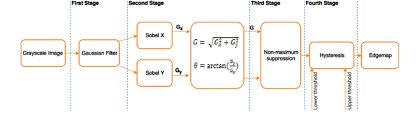
\includegraphics[width=1.0\textwidth]{images/canny_edge_detection_steps.png}
    \captionof{figure}{Các bước của thuật toán phát hiện biên Canny. (a) Ảnh gốc. (b) Làm mờ bằng bộ lọc Gaussian. (c) Tính toán độ lớn gradient, làm nổi bật các cạnh. (d) Áp dụng Non-maximum Suppression để làm mỏng các cạnh. (e) Kết quả cuối cùng sau khi áp dụng Hysteresis Thresholding.}
    \label{fig:canny_steps}
\end{center}

Các bước của thuật toán Canny:
\begin{enumerate}
    \item \textbf{Khử nhiễu (Noise Reduction):} Bước đầu tiên luôn là làm mờ ảnh bằng bộ lọc Gaussian để loại bỏ nhiễu, vì các phép toán đạo hàm rất nhạy cảm với nhiễu. Kích thước của kernel Gaussian ($\sigma$) là một tham số quan trọng: $\sigma$ lớn sẽ giảm nhiễu tốt hơn nhưng có thể làm mất các cạnh yếu.
    
    \item \textbf{Tìm Độ lớn và Hướng Gradient:} Sử dụng các bộ lọc Sobel (hoặc các bộ lọc tương tự) để tính toán gradient theo hướng $x$ ($G_x$) và $y$ ($G_y$). Từ đó, tính độ lớn gradient $G = \sqrt{G_x^2 + G_y^2}$ và hướng gradient $\theta = \arctan(G_y / G_x)$ cho mỗi pixel. Hướng gradient này luôn vuông góc với hướng của cạnh.
    
    \item \textbf{Non-maximum Suppression (Loại bỏ các điểm không phải cực đại):} Bước này nhằm mục đích làm cho các cạnh trở nên mỏng, chỉ còn 1 pixel. Các cạnh được tạo ra từ bước 2 thường dày và mờ. Ý tưởng là: một pixel chỉ được coi là cạnh nếu giá trị độ lớn gradient của nó là \textit{cực đại cục bộ} theo hướng gradient.
    
    Quy trình: Đối với mỗi pixel, ta xem xét hướng gradient $\theta$ của nó. Hướng này được làm tròn thành một trong bốn hướng chính (0°, 45°, 90°, 135°). Sau đó, ta so sánh độ lớn gradient của pixel hiện tại với hai pixel lân cận nằm trên đường thẳng theo hướng gradient đó. Nếu giá trị của pixel hiện tại không lớn hơn cả hai lân cận, nó sẽ bị loại bỏ (đặt bằng 0). Kết quả là một ảnh các cạnh mỏng.
    
    \item \textbf{Hysteresis Thresholding (Ngưỡng Kép và Liên kết):} Đây là bước thông minh nhất của thuật toán Canny. Thay vì sử dụng một ngưỡng duy nhất, nó sử dụng hai ngưỡng: một ngưỡng cao ($T_{\text{high}}$) và một ngưỡng thấp ($T_{\text{low}}$).
    \begin{itemize}
        \item Các pixel có độ lớn gradient lớn hơn $T_{\text{high}}$ được coi là \textbf{cạnh mạnh (strong edges)} và chắc chắn là một phần của đường biên cuối cùng.
        \item Các pixel có độ lớn gradient nhỏ hơn $T_{\text{low}}$ được coi là không phải cạnh và bị loại bỏ.
        \item Các pixel có độ lớn gradient nằm giữa $T_{\text{low}}$ và $T_{\text{high}}$ được coi là \textbf{cạnh yếu (weak edges)}. Một cạnh yếu chỉ được giữ lại nếu nó \textbf{kết nối} với một cạnh mạnh, trực tiếp hoặc gián tiếp thông qua các cạnh yếu khác.
    \end{itemize}
    \textbf{Trực giác:} Các cạnh mạnh được coi là những điểm "chắc chắn" là cạnh. Sau đó, thuật toán sẽ "bám" theo những điểm này để nối các phần yếu hơn của cùng một đường biên, trong khi vẫn loại bỏ được các điểm nhiễu đơn lẻ có độ lớn gradient nằm trong khoảng giữa hai ngưỡng. Kỹ thuật này giúp giải quyết được sự đánh đổi giữa việc phát hiện các cạnh yếu và việc tạo ra các cạnh giả do nhiễu.
\end{enumerate}

Thuật toán Canny, với sự kết hợp của lọc Gaussian, non-maximum suppression và hysteresis thresholding, tạo ra các bản đồ cạnh chất lượng cao, mỏng và ít bị đứt gãy.


\subsection{Các phép toán Hình thái học (Morphological Operations)}
\label{subsec:morphological_operations}

Trong khi các phép lọc dựa trên tích chập là các phép toán số học, \textbf{xử lý ảnh hình thái học (morphological image processing)} \cite{Serra1982} là một bộ công cụ mạnh mẽ dựa trên \textbf{lý thuyết tập hợp (set theory)}. Nó thường được áp dụng trên ảnh nhị phân (binary images) hoặc ảnh xám để xử lý và phân tích \textit{hình dạng (shape)} của các đối tượng.

\subsubsection{Các khái niệm Cơ bản: Tập hợp và Phần tử Cấu trúc}
\label{subsubsec:morpho_basics}
Trong xử lý hình thái học nhị phân, các pixel có giá trị 1 (foreground) được xem như các phần tử của một tập hợp. 
\begin{equation}
    A = \{ (x, y) \mid I[x, y] = 1 \}
\end{equation}
Mọi phép toán hình thái học đều được định nghĩa dựa trên sự tương tác giữa tập hợp pixel ảnh $A$ và một tập hợp nhỏ khác gọi là \textbf{phần tử cấu trúc (Structuring Element - SE)}, ký hiệu là $B$.

Phần tử cấu trúc hoạt động tương tự như kernel trong phép tích chập. Nó là một mẫu hình dạng nhỏ (ví dụ: hình vuông, hình tròn, hình chữ thập) trượt qua ảnh. Hình dạng và kích thước của SE quyết định hiệu ứng của phép toán. Mỗi SE có một \textbf{điểm gốc (origin)} hay điểm neo.

\begin{center}
    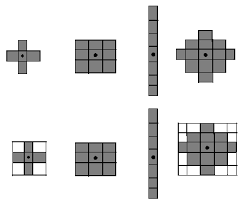
\includegraphics[width=0.7\textwidth]{images/structuring_elements.png}
    \captionof{figure}{Một số ví dụ về phần tử cấu trúc như hình vuông, hình chữ thập, hình đĩa. Hình dạng và kích thước của SE được chọn để phù hợp với hình dạng của đối tượng cần xử lý.}
    \label{fig:structuring_elements}
\end{center}

\subsubsection{Hai phép toán Cơ bản: Co (Erosion) và Giãn (Dilation)}
\label{subsubsec:erosion_dilation}
Đây là hai phép toán nền tảng của xử lý hình thái học.

\begin{description}
    \item[Phép Co (Erosion - $\ominus$):] Trực giác, phép co "làm mòn" hoặc "co rút" các đối tượng trong ảnh. Về mặt toán học, phép co của tập $A$ bởi SE $B$ được định nghĩa là tập hợp tất cả các điểm $z$ sao cho khi dịch chuyển $B$ đến $z$ (đặt gốc của $B$ tại $z$), $B$ được \textbf{chứa hoàn toàn} trong $A$.
    \begin{equation}
        A \ominus B = \{ z \mid (B)_z \subseteq A \}
    \end{equation}
    \textbf{Tác dụng:}
    \begin{itemize}
        \item Loại bỏ các đối tượng nhỏ, nhiễu "muối" (các pixel trắng đơn lẻ).
        \item Tách các đối tượng bị dính liền với nhau bởi các cầu nối mỏng.
        \item Thu nhỏ kích thước của tất cả các đối tượng.
    \end{itemize}
    
    \item[Phép Giãn (Dilation - $\oplus$):] Trực giác, phép giãn "làm phình to" hoặc "giãn nở" các đối tượng. Phép giãn của $A$ bởi $B$ được định nghĩa là tập hợp tất cả các điểm $z$ sao cho khi dịch chuyển $B$ đến $z$, giao của nó với $A$ \textbf{không rỗng}.
    \begin{equation}
        A \oplus B = \{ z \mid (\hat{B})_z \cap A \neq \emptyset \}
    \end{equation}
    Trong đó $\hat{B}$ là phép phản xạ của $B$ qua gốc của nó. Trực giác hoạt động của nó là trượt SE $B$ qua ảnh $A$, và tại mỗi vị trí mà SE "chạm" vào một pixel của đối tượng, toàn bộ vùng mà SE bao phủ sẽ được "bật" lên thành 1 ở ảnh đầu ra.
    \textbf{Tác dụng:}
    \begin{itemize}
        \item Lấp đầy các lỗ nhỏ hoặc các vết nứt bên trong đối tượng.
        \item Nối liền các phần bị đứt gãy của một đối tượng.
        \item Làm tăng kích thước của tất cả các đối tượng.
    \end{itemize}
\end{description}

\begin{center}
    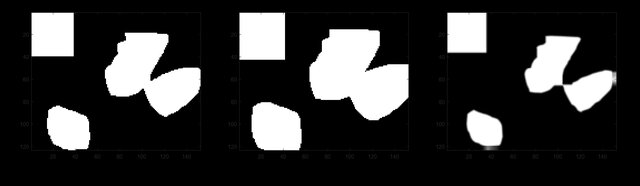
\includegraphics[width=1.0\textwidth]{images/erosion_dilation.jpg}
    \captionof{figure}{Minh họa phép Co và Giãn. (a) Ảnh nhị phân gốc. (b) Kết quả sau phép Co, các đối tượng bị thu nhỏ và các chi tiết nhỏ bị loại bỏ. (c) Kết quả sau phép Giãn, các đối tượng phình to và các lỗ nhỏ được lấp đầy.}
    \label{fig:erosion_dilation_example}
\end{center}

\subsubsection{Các phép toán Phức hợp: Mở (Opening) và Đóng (Closing)}
\label{subsubsec:opening_closing}
Phép co và giãn làm thay đổi kích thước của đối tượng. Để thực hiện các thao tác lọc hình thái mà không làm thay đổi kích thước tổng thể, người ta kết hợp hai phép toán này.

\begin{description}
    \item[Phép Mở (Opening - $\circ$):] Là phép \textbf{co} theo sau bởi một phép \textbf{giãn} với cùng một phần tử cấu trúc.
    \begin{equation}
        A \circ B = (A \ominus B) \oplus B
    \end{equation}
    \textbf{Trực giác:} Phép co ban đầu sẽ loại bỏ các "bán đảo" mỏng, các cầu nối hẹp và các chấm nhiễu nhỏ. Phép giãn sau đó sẽ khôi phục lại kích thước của các đối tượng chính đã bị co lại, nhưng nó không thể khôi phục lại những gì đã bị loại bỏ hoàn toàn. Giống như việc "lăn" phần tử cấu trúc \textit{bên trong} đường viền của đối tượng; những chỗ nào SE không lọt vào được sẽ bị loại bỏ.
    \textbf{Tác dụng:}
    \begin{itemize}
        \item Làm mượt đường viền của đối tượng.
        \item Loại bỏ các phần nhô ra mỏng (protrusions).
        \item Tách các đối tượng bị dính liền.
    \end{itemize}
    
    \item[Phép Đóng (Closing - $\bullet$):] Là phép \textbf{giãn} theo sau bởi một phép \textbf{co} với cùng một phần tử cấu trúc.
    \begin{equation}
        A \bullet B = (A \oplus B) \ominus B
    \end{equation}
    \textbf{Trực giác:} Phép giãn ban đầu sẽ lấp đầy các lỗ nhỏ và các vết nứt. Phép co sau đó sẽ thu nhỏ các đối tượng về lại kích thước ban đầu, nhưng các lỗ đã được lấp đầy sẽ không xuất hiện trở lại. Giống như việc "lăn" phần tử cấu trúc \textit{bên ngoài} đường viền của đối tượng; những "vịnh" hay "khe hở" nào mà SE không lọt vào được sẽ bị lấp đầy.
    \textbf{Tác dụng:}
    \begin{itemize}
        \item Làm mượt đường viền.
        \item Lấp đầy các lỗ nhỏ bên trong đối tượng.
        \item Nối liền các đoạn bị đứt gãy.
    \end{itemize}
\end{description}

\begin{center}
    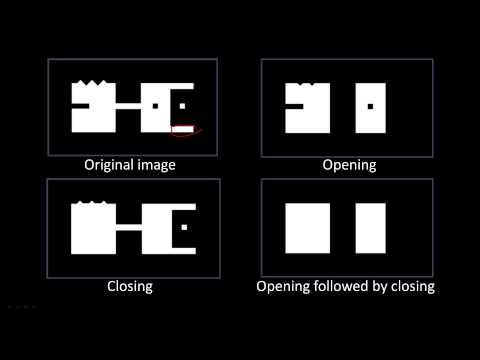
\includegraphics[width=1.0\textwidth]{images/opening_closing.jpg}
    \captionof{figure}{Minh họa phép Mở và Đóng. (a) Ảnh gốc có nhiễu muối (điểm trắng) và nhiễu tiêu (lỗ đen). (b) Phép Mở loại bỏ các điểm nhiễu trắng nhưng giữ lại các lỗ. (c) Phép Đóng lấp đầy các lỗ đen nhưng giữ lại các điểm nhiễu. (d) Mở rồi Đóng (hoặc ngược lại) có thể loại bỏ cả hai loại nhiễu.}
    \label{fig:opening_closing_example}
\end{center}

Các phép toán hình thái học là những công cụ cực kỳ hiệu quả để tiền xử lý ảnh nhị phân trước các bước như trích xuất đặc trưng hình dạng hoặc đếm đối tượng.

\section*{Kết luận}
Qua phần này, chúng ta đã khám phá hai họ công cụ cơ bản nhưng cực kỳ mạnh mẽ trong xử lý ảnh: các phép lọc dựa trên tích chập và các phép toán hình thái học. Tích chập, với khả năng thực hiện các phép toán cục bộ có trọng số, là nền tảng cho việc làm mờ (lọc thông thấp) để giảm nhiễu và làm sắc nét (lọc thông cao) để tăng cường chi tiết. Đỉnh cao của các kỹ thuật dựa trên đạo hàm là thuật toán Canny, một quy trình nhiều bước tinh vi để trích xuất các đường biên một cách chính xác và mạnh mẽ. Mặt khác, các phép toán hình thái học, dựa trên lý thuyết tập hợp, cung cấp một bộ công cụ hoàn toàn khác để phân tích và thao tác hình dạng của các đối tượng. Các phép toán cơ bản như co, giãn và các phép toán phức hợp như mở, đóng cho phép chúng ta dọn dẹp nhiễu, tách/nối các đối tượng và đơn giản hóa hình dạng một cách hiệu quả.
Việc nắm vững cả hai bộ công cụ này—một hoạt động trên giá trị pixel, một hoạt động trên hình dạng—là điều kiện cần để xây dựng các pipeline xử lý ảnh cổ điển vững chắc và cũng là để hiểu sâu hơn về các cơ chế hoạt động bên trong các mạng nơ-ron hiện đại.

\section*{Tài liệu tham khảo}
\begin{itemize}
	\item Gonzalez, R. C.; Woods, R. E. \textit{Digital Image Processing}. 4th ed. Pearson, 2018. (Chương 3 và 9 về lọc ảnh và xử lý hình thái học).
	\item Canny, J. A Computational Approach to Edge Detection. \textit{IEEE Transactions on Pattern Analysis and Machine Intelligence} \textbf{1986}, \textit{PAMI-8}(6), 679–698.
	\item Serra, J. \textit{Image Analysis and Mathematical Morphology}. Academic Press, 1982.
	\item Bhardwaj, S.; Mittal, A. A Survey on Various Edge Detector Techniques. \textit{Procedia Technology} \textbf{2012}, \textit{4}, 220-226.
	\item Abushaala, A. M. Edge detection methods. In \textit{2nd IEEE World Symposium on Web Applications and Networking (WSWAN)}, 2015.
	\item Jain, A. K. \textit{Fundamentals of Digital Image Processing}. Prentice Hall, 1989.
	\item Pratt, W. K. \textit{Digital Image Processing: PIKS Scientific Inside}. 4th ed. Wiley, 2007.
	\item Lim, J. S. \textit{Two-Dimensional Signal and Image Processing}. Prentice Hall, 1990.
	\item Gonzalez, R. C.; Woods, R. E.; Eddins, S. L. \textit{Digital Image Processing Using MATLAB}. 3rd ed. Gatesmark, 2018.
	\item Castleman, K. R. \textit{Digital Image Processing}. Prentice Hall, 1996.
	\item Russ, J. C. \textit{The Image Processing Handbook}. 7th ed. CRC Press, 2016.
	\item Burger, W.; Burge, M. J. \textit{Digital Image Processing: An Algorithmic Introduction Using Java}. Springer, 2009.
	\item Sonka, M.; Hlavac, V.; Boyle, R. \textit{Image Processing, Analysis, and Machine Vision}. 4th ed. Cengage, 2014.
	\item Gonzalez, R. C.; Woods, R. E. \textit{Digital Image Processing}. 4th ed. Pearson, 2018. (Chương 4 về lọc không gian tần số).
	\item Marr, D.; Hildreth, E. Theory of Edge Detection. \textit{Proceedings of the Royal Society B}, 1980, 207, 187–217.
	\item Canny, J. Edge detection techniques revisited. \textit{International Journal of Computer Vision}, 2013, 102, 1–25.
	\item Gonzalez, R. C.; Woods, R. E. \textit{Digital Image Processing}. 4th ed. Pearson, 2018. (Chương 5 về tăng cường ảnh).
	\item Soille, P. \textit{Morphological Image Analysis: Principles and Applications}. 2nd ed. Springer, 2003.
	\item Dougherty, E. R.; Lotufo, R. A. \textit{Hands-on Morphological Image Processing}. SPIE Press, 2003.
	\item Vincent, L. Morphological Grayscale Reconstruction in Image Analysis. \textit{Computer Vision and Image Understanding}, 1993, 64(2), 199–223.
\end{itemize}
